\chapter{Background}\label{ch:background}
As discussed in Chapter 1, reductive evolution is a  

\section{Experimental Evolution}
As discussed in Section \ref{problem_statement}, in vivo experiments, although sometimes more realistic, have their own set of difficulties. Some examples of these difficulties include recreating challenging environmental conditions (e.g. simulating the open ocean in a lab) and identifying and/or simulating the multiple selection pressures acting on genomes in the real world \cite{Batut.2013}. These challenges add enormous difficulty and complexity to conducting proper experiments and isolating the specific factors which lead to particular outcomes. 

In silico evolution simulates organisms in software, thus allowing for far greater control and analysis of the environment and other experimental conditions. In contrast to in vivo experiments, a greater amount of control is also available with regard to the way organisms may interact, reproduce, and evolve. For example, a genome may be created completely from scratch or an existing genome may be fed into the simulation. Reproduction rates can depend on overall fitness, on relative fitness, or some other criterion.

Factors such as the mutation rates or selection pressure are then parameters for the model and may be kept constant or allowed to vary over time. Given that these are parameters of the system, they may be tightly controlled, leading to a clearer picture of the factors influencing different outcomes. An underlying deterministic model can also allow for a reconstruction of the system from any given point, allowing one to easily create a record of events, including phylogenetic trees. 

\subsubsection{Why use Aevol}
The in silico tool \textit{Aevol} was developed in the early 2000s to ``study the evolution of the size and organization of bacterial genomes in various scenarios''\cite{Batut.2013}. The program has been expanded upon and tested in a variety of scenarios over the years. Examples of such experiments include: testing the predictability of evolution with high mutation rates as in viruses, \cite{beslon:hal-01577115}, determining whether selection is able to overcome evolution's drive towards more complex organisms \cite{doi:10.1162}, examining the role of mutators in reorganizing the genome in order to overcome mutational load \cite{doi:10.1186/s12862-019-1507-z}, examining the effects of population shape on levels of cooperation \cite{doi:10.1162/978-0-262-33936-0-ch057}, modeling regulatory networks \cite{sanchezdehesa:hal-01502737} and more. 
 
In the following sections, the in silico experimental evolution tool Aevol will be examined in greater detail. 

\section{Aevol}
Organisms are simulated with a binary genome which can either be generated at random or input as a previously-generated sequence. Aevol essentially consists of three steps: 1) decoding the genome of these organisms to produce artificial proteins, 2) selecting the most fit individuals and 3) reproduction of these fittest individuals with possible variations (mutations, rearrangements, etc.). The population size $N$ is kept constant and a record of each generation is kept so that the phylogenetic lineages can be recreated.

\subsection{Aevol's Architecture}
Aevol's three steps\textemdash decoding the genome, selection, and reproduction\textemdash will be examined in more detail in this section. These steps are illustrated in Figure \ref{fig:aevol_overview01}. 

\begin{figure}[H]\label{fig:aevol_overview01}
	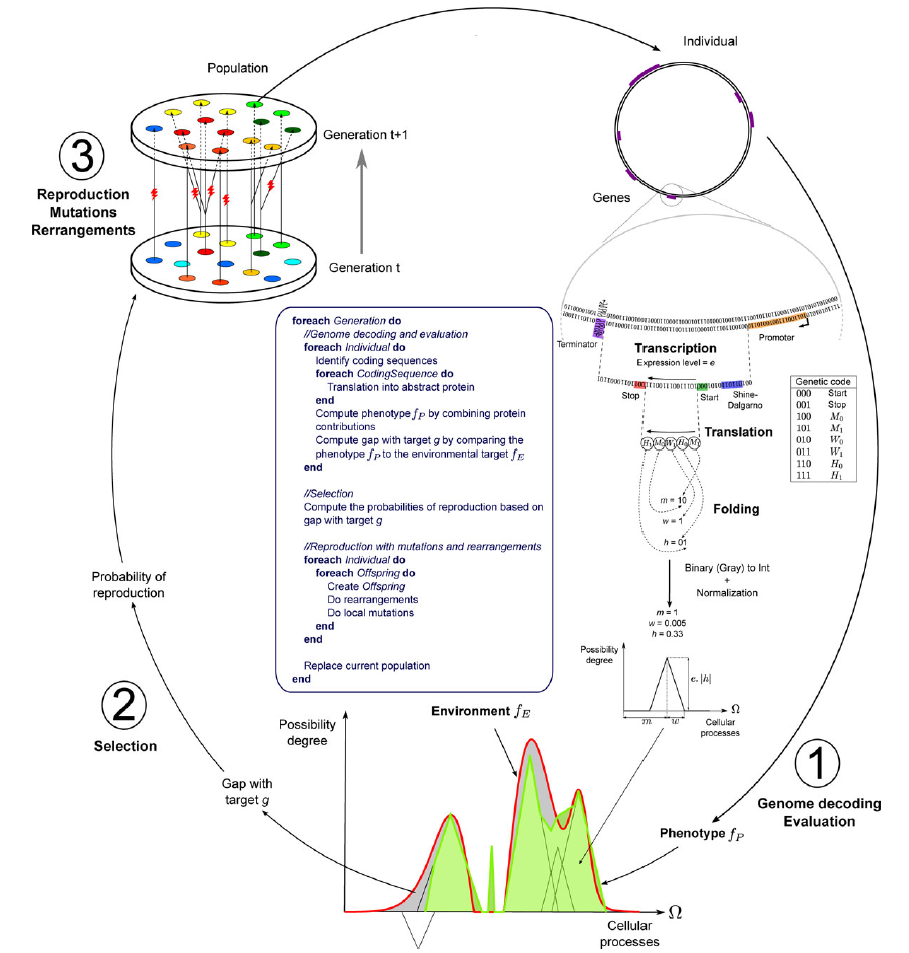
\includegraphics[scale=0.65]{aevol_overview01}
	\centering
	\caption[Overview of Aevol's architecture.]{Overview of Aevol's architecture, from \cite{Batut.2013}}
\end{figure}
\subsubsection{Decoding the Genome}
In Aevol, a genome consists of a string of binary characters where 0 is complementary to 1. Each organism in the (initially clonal) population has a double-stranded circular genome which is either generated randomly or which was provided as input. To decode the genome and produce the phenotype, the sequence is searched for transcribed regions. Transcribed regions are denoted by promoter and terminator sequences. The promoter sequence is a sequence whose Hamming distance $d$ is within $d_{max} = 4$ mismatches of the predefined consensus sequence $0101011001110010010110$. Terminators are sequences which can form a stem-loop structure with a stem size of 4 bases and a loop length of 3 bases (i.e. $abcd$***$\overline{dcba}$ where a is complementary to $\overline{a}$, b is complementary to $\overline{b}$, etc.). Lastly, the initiation and termination signals are sought, which are simply Shine-Dalgarno-like signals (i.e. $011011****000$ to start and $011011****001$ to stop). Lastly, an expression level $e$ is assigned to each coding region, following the formula $e = 1 - \frac{d}{d_{max} + 1}$ where $d$ is again the Hamming distance between the coding region and the consensus sequence given above and $d_{max}$ is the maximum allowable distance (i.e. 4). 

Once an initiation sequence is found, the following bases are read three at a time (codon by codon) until a stop codon (by default $001$) is found. If a stop codon is not found, then no protein is produced. Since a transcribed region may have multiple initiation signals, operons are therefore allowed. The codons following an initiation signal encode for three parameters according to the genetic code given in Figure \ref{fig:aevol_overview01}: $m$ (mean), $w$ (half-width), and $h$ (height), which together define a triangle representing a ``cellular process''.

A cellular process is simply an abstract representation of some phenotypic function and is represented by the ordered set $\Omega = \left[ a,b \right] \subset \mathbb{R}$. To keep things simple, $\Omega$ is a one-dimensional space in the interval $\left[0,1\right]$, i.e. a ``cellular process'' is simply a real number, and the genomic encoding of each cellular process determines the function $f(x) : \Omega \rightarrow \left[0,1\right]$. The mean $m$ gives us the specific cellular process in the range $\left[0,1\right]$. The width $w$ describes the ``scope'' of the process, i.e. the \textit{pleiotropy} of the process, meaning the subset of the protein that is in the interval $ \left(m - w, m + w\right) \subset \Omega$ . The height determines the degree of possibility of the process, i.e. its relative strength.

The codons are read one after the other and their Gray codes\footnote{A binary encoding such that two successive values (e.g. 2, 3) only differ by at most one bit (e.g. 0011, 0010). See \url{https://en.wikipedia.org/wiki/Gray_code}} are used to compute the real numbers $m$, $w$, and $h$ as follows. Each parameter ($m$, $w$, $h$) is assigned two codons in the genetic code (see Figure \ref{fig:aevol_overview01}), for example $w_0 = 010$ and $w_1 = 011$. Any $w_0$ codons become a $0$ in the Gray code, and vice versa with $1$s. So if, for example, when reading the coding sequence, the codons $w_1$, $w_0$, $w_1$, $w_0$ are read, the Gray code becomes $1010$, which is 12 in decimal. This is done for $m$, $w$, and $h$, and the resulting values are then normalized to be in the proper range. $w$'s range is specified in the parameter file (\texttt{MAX\_TRIANGLE\_WIDTH}), $h$ must be in the range $\left[-1,+1\right]$ (indicating that both activating and inhibitive processes are allowed) and $m$ must be in the range $\left[0,1\right]$ (the range of $\Omega$). 

Given multiple coding sequences in a genome, several triangles are translated from the genome, each parameterized by its own $m$, $w$, and $h$. These triangles form the phenotypic function $f_P$. \textit{Fuzzy logic} is used to find the overall contribution of each cellular process, using the Lukasiewicz fuzzy operators\footnote{See \url{https://en.wikipedia.org/wiki/Lukasiewicz\_logic} for an introduction.}. In short, the activating proteins are added up, as are the inhibiting proteins, and the difference between these two totals represents the final function $f_P$. 

\subsubsection{Selection}
After the genome is decoded, the organisms are tested for their fitness. Fitness in Aevol is defined as the gap between the phenotype of a sequence $f_P$ and the environmental  target function $f_E$, as illustrated in Figure \ref{fig:aevol_overview01}. This environmental target function $f_E$ is a user-determined set of Gaussians which are specified in a parameter file. The difference between the phenotype (as calculated above) and the environmental function is the ``metabolic error'', labeled $g$ in the Figure and is more formally defined as:  $g = \int_{a}^{b} f_E(x) - f_P(x) dx$.

Aevol contains several selection schemes but here we will only consider the \texttt{fitness\_proportionate} scheme, since this was the only selection scheme employed in our experiments. In this scheme, the probability of reproduction for each organism is proportionate to its fitness, namely $P(\text{reproduction}) = exp(-k * g)$, where $k$ is a user-definable parameter which determines the selection intensity and $g$ is the metabolic error.
\subsubsection{Reproduction}
Once the fittest organisms in the population are found and their probabilities of reproducing are calculated as described in the previous Section, new organisms are produced by drawing from a multinomial distribution. Since the population size is held constant, this implies that a single organism with a high probability of reproduction may produce multiple offspring and an organism with low probability of reproduction may produce none.

When new organisms are created and their genomes are copied from their parent organisms, it is at this stage that the driving force in evolution occurs, namely the possibility for mutation, indels, and frameshifts. Mutation rates are set in the parameter file and include point mutations, insertions and deletions (indels), and rearrangements (duplication, deletions, translocations, and inversions).

The mutation, indels, rearrangement, etc. events are carried out by first determining the number $\mu$ of such events which will occur, based on the mutation rate specified in the parameter file and drawing from a binomial distribution (e.g. $B(L, \mu_\text{point})$ for point mutations, $B(L, \mu_\text{large deletions})$ for large deletions, etc. where $L$ is the size of the genome). Then a random point (or points, in the case of e.g. rearrangement) is chosen and the event is carried out, with the order of events shuffled randomly. 
\subsection{Aevol's Statistics and Post-Treatments}\label{aevol_post-treatments}
Aevol by default produces several statistics files which include information about genome size, the percentage of coding DNA, number of genes, average metabolic error, and many other factors.  It further includes a number of post-treatments that allow one to analyze specific individuals or the population at large, including tools for determining robustness, evolvability, coalescence, and the lineages. 

In the following two subsections we will examine evolvability and robustness, as these two factors play a major role in reductive evolution. 

\subsubsection{Evolvability}
Evolvability is usually defined as the ability of a system (in this case an organism) to evolve. In other words, ``if mutations in it can produce heritable phenotypic variation''\cite{doi:10.1098/rspb.2007.1137}. However, of critical importance is that this is not simply having a large amount of genetic diversity, but rather \textit{adaptive} diversity which provides some benefit. 

It is a seeming trade-off between robustness and evolvability. The more robust a system is, the less phenotypic variation is generated by random mutation events, and thus less evolvability. 

\subsubsection{Robustness}


\subsubsection{aevol\_misc\_ancestor\_mutagenesis}
This post-treatment generates and analyses mutants for the provided lineage. Specifically, this program generates evolvability, robustness, and antirobustness statistics for the mutants. 

\subsubsection{aevol\_misc\_ancestor\_robustness}
Generates mutants for a given lineage and analyzes their robustness, providing several statistics:



\subsubsection{aevol\_misc\_ancestor\_stats}

Analyzes a lineage and produces the following outputs:



\subsubsection{aevol\_misc\_coalescence}
Prints coalescence statistics for a given lineage.

\subsubsection{aevol\_misc\_create\_eps}
Creates a directory, analysis-generation\_XXXXX with several EPS files.The EPS files are as follows:


\subsubsection{aevol\_misc\_extract}

Extracts the genotype and/or data about the phenotype of individuals in the provided population and write them into text files for easy parsing by programs such as MATLAB. The program lets you specify whether you want the sequence, the triangle data, or both. By default (i.e. with no parameters) gives just the sequence, into a file called “sequence”.

\subsubsection{aevol\_misc\_lineage}

Using the tree files, recreates the lineage of an individual. By default, this is done for the best individual, but another individual can be specified by ID number or rank (-i or -r, respectively). 

\subsubsection{aevol\_misc\_mutagenisis}

This generates and analyzes mutations for an individual from a population backup (as opposed to a lineage file for ancestor\_mutagenesis). One can specify point mutations, small indels, duplications, large deletion, translocations, or inversions. 

\subsubsection{aevol\_misc\_protein\_map}

Creates a CSV file which analyzes the proteins generated by the specified lineage. The CSV file specifies:



\subsubsection{aevol\_misc\_robustness}

Calculates replication statistics for a given individual (specified by either ID or rank) at a given time.  Specifically, the following information is saved in a new directory (analysis-generation\_XXXXXXXXXX):


\section{Changeable Factors}
\subsection{Fitness}
\subsection{Evolvability}
\subsection{Robustness}
\subsection{Structure}
\subsubsection{Percent Coding vs. Non-Coding DNA}
\subsubsection{Number of Genes}


\section{Related Work}\label{related_work}
